\section{Results and Discussion}

\begin{figure}[h!]
    \centering
    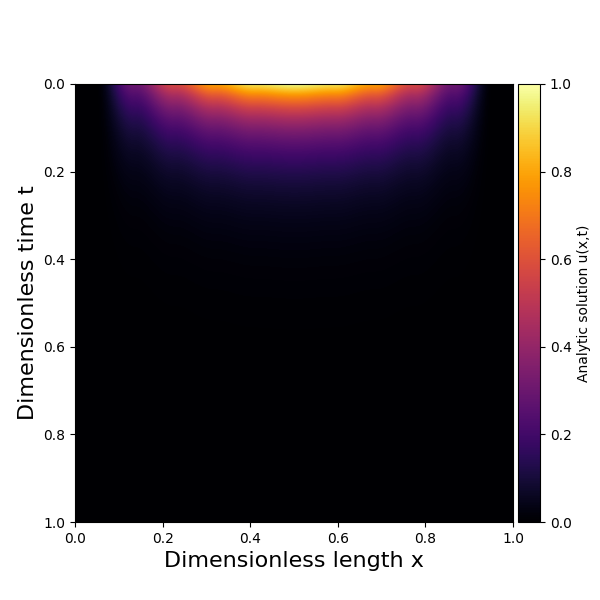
\includegraphics[width=8cm]{../Figures/analytic_solution.png}
    \caption{Analytic solution for the heat equation with initial conditions
    $u(x,0)=\sin{(\pi x)}$ and boundary conditions $u(0,t)=u(1,t)=0$.}
    \label{fig:analytic_solution}
\end{figure}

In figure \ref{fig:analytic_solution} we see the analytic solution for our
given boundary and initial conditions. This will be used to test our numerical
solvers using the absolute error between this and the numerical approximation.
This can be seen in figure \ref{fig:abs_error_all}. In the subfigures (a)-(d)
we see the NNs prediction for different activation functions and optimizers. We
can see that ReLu with RMSprop has the lowest error. And we note that all of
the approximations have the highest loss at the boundaries. We can especially
see that Adam with ReLu has a very high error at the $t=0$ boundary. The reason
our network is not handling the boundaries well is because the loss function
has no special penalizing of wrong boundaries. This could be fixed by creating
a new loss function by looking at the minimization of the NNs prediction

\begin{equation*}
    \min_{\hat{u}} \left\{
    \lVert \hat u_{xx} - \hat u_t \rVert^2 
    + \lVert \hat u(0,t) \rVert^2 
    + \lVert \hat u(1,t) \rVert^2
    + \lVert \hat u(x,0)-\sin{(\pi x)}\rVert^2 \right\},
\end{equation*}
where this norm $\lVert \cdot \rVert$ is to be read as the grand sum of the
matrix. We then define our cost/loss-function as
\begin{equation*}
    C(\hat u) =\frac{1}{2} \left[ \lVert \hat u_{xx} - \hat u_t \rVert^2 
    + \lVert \hat u(0,t) \rVert^2 
    + \lVert \hat u(1,t) \rVert^2
    + \lVert \hat u(x,0)-\sin{(\pi x)}\rVert^2 \right].
\end{equation*}
We can then add parameters in front of the norms to decide how costly it would
be for the network to not prioritize the boundaries. This is called a physics
informed neural network and has been explored in a previous paper (Zobeiry \&
Humfeld, 2020)\cite{2}. Getting back to figure \ref{fig:abs_error_all}, we look
at the explicit solver in (e). Note here that the limits on the colorbar is
changed because the error is so small compared to that of the NNs. We see that
now our boundaries is forced to be correct. And we can see that as we move in
time the middle of the rod gets a larger and larger error until it starts
cooling down and of course the error gets smaller because the values get closer
and closer to zero because of the $u(0,t)=u(1,t)=0$ boundaries.

!!!YOU STOPPED HERE!!! Next is loss vs epochs for all methods. Then loss vs
layers. Then time vs matrixsise


\begin{figure}
\centering
\subfigure[Rms, ReLu]{\label{fig:a}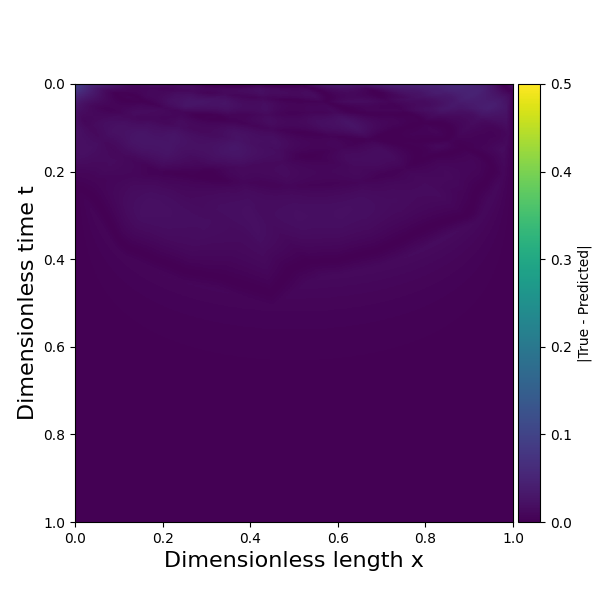
\includegraphics[width=70mm]{../Figures/error_rms_relu.png}}
\subfigure[Rms, Sigmoid]{\label{fig:b}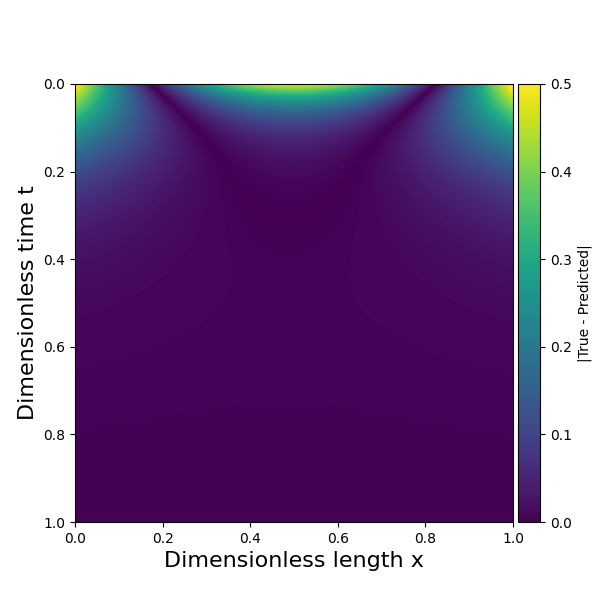
\includegraphics[width=70mm]{../Figures/error_rms_sigmoid.png}}
\subfigure[Adam, ReLu]{\label{fig:c}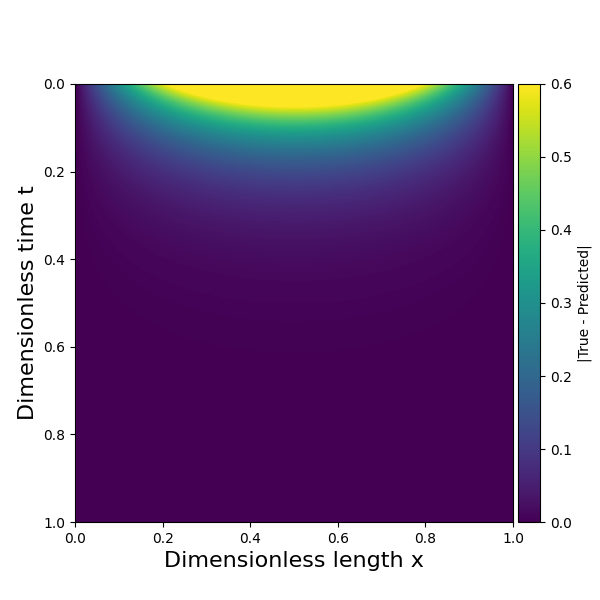
\includegraphics[width=70mm]{../Figures/error_adam_relu.png}}
\subfigure[Adam, Sigmoid]{\label{fig:d}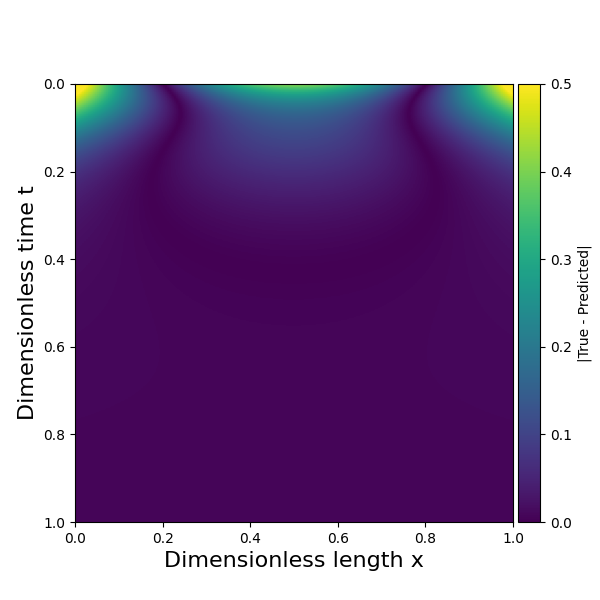
\includegraphics[width=70mm]{../Figures/error_adam_sigmoid.png}}
\subfigure[Explicit solver]{\label{fig:e}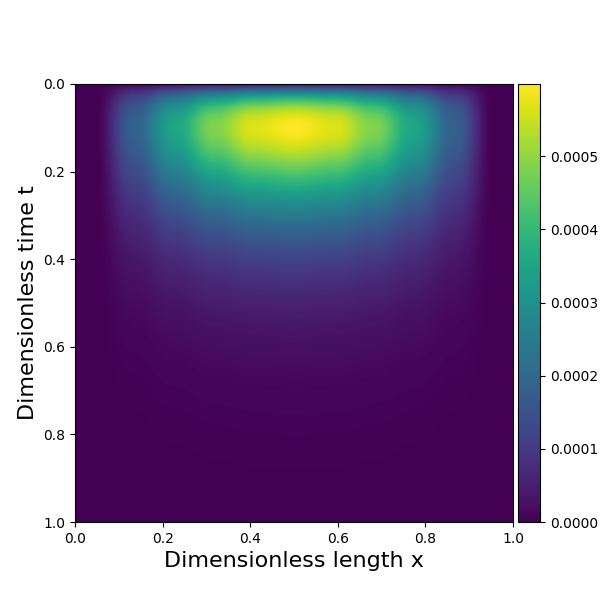
\includegraphics[width=70mm]{../Figures/error_explicit.png}}
\caption{Absolute error for NN in (a)-(d) and explicit solver in (e). NN is
trained with 20 epochs and a batch size of 30 with $(n=100)\times (m=100)$
data points of $x$
and $t$ respectively, using the analytical solution for MSE as the loss
function. The explicit solver in (e) is using $\Delta x=0.1$ and $\alpha=1/4$.}
\label{fig:abs_error_all}
\end{figure}
